\documentclass[10pt,a4paper,landscape]{article}

\usepackage[utf8]{inputenc}
\usepackage[T1]{fontenc}
\usepackage{lmodern}
\usepackage[landscape,margin=1.35cm]{geometry}
\usepackage{underscore}
\usepackage{amsmath}
\usepackage{array}
\usepackage{booktabs}
\usepackage{longtable}
\usepackage{colortbl}
\usepackage{xcolor}
\usepackage{tikz}
\usetikzlibrary{calc,positioning,shapes.geometric,arrows.meta}
\usepackage{enumitem}
\usepackage{float}
\usepackage{fancyhdr}
\usepackage{titlesec}
\usepackage{caption}
\usepackage[hidelinks]{hyperref}

\hypersetup{
  pdftitle={Farmacia Lufar - Modelo Entidad-Relacion y Modelo Relacional},
  pdfauthor={Documento de diseno de base de datos},
  pdfsubject={Modelo de datos para el sistema de gestion de Farmacia Lufar}
}

\definecolor{azulEnt}{HTML}{E8F1FB}
\definecolor{verdeEnt}{HTML}{EAF5EA}
\definecolor{naranjaEnt}{HTML}{FFF0E0}
\definecolor{violetaEnt}{HTML}{F2EAF8}
\definecolor{grisEnt}{HTML}{F0F0F0}
\definecolor{grisConfig}{HTML}{F7F7F7}

\pagestyle{fancy}
\fancyhf{}
\fancyhead[L]{\sffamily\small Farmacia Lufar}
\fancyhead[R]{\sffamily\small Modelo de base de datos}
\fancyfoot[C]{\sffamily\small\thepage}
\renewcommand{\headrulewidth}{0.4pt}

\setlength{\parindent}{0pt}
\setlength{\parskip}{4pt}
\renewcommand{\arraystretch}{1.18}

\newcommand{\code}[1]{\texttt{\detokenize{#1}}}
\newcommand{\pk}[1]{\underline{\code{#1}}}
\newcommand{\fk}[1]{\textbf{\code{#1}}}
\newcommand{\uk}{\textsuperscript{\textsc{uk}}}

\tikzset{
  entity/.style={
    draw=black!65,
    rounded corners=2.5pt,
    thick,
    align=left,
    inner sep=3.5pt,
    font=\sffamily\scriptsize,
    fill=white,
    minimum height=1.0cm
  },
  catalogo/.style={entity, fill=azulEnt},
  compras/.style={entity, fill=verdeEnt},
  inventario/.style={entity, fill=naranjaEnt},
  ventas/.style={entity, fill=violetaEnt},
  seguridad/.style={entity, fill=grisEnt},
  configuracion/.style={entity, fill=grisConfig},
  rel/.style={draw=black!60, thick, rounded corners=4pt},
  card/.style={font=\sffamily\scriptsize, fill=white, inner sep=1pt},
  lbl/.style={font=\sffamily\scriptsize\itshape, fill=white, inner sep=1pt}
}

\newcommand{\rel}[5]{%
  \draw[rel] (#1) --
    node[pos=0.25, above, card] {#2}
    node[pos=0.75, above, card] {#3}
    node[midway, below, lbl] {#4} (#5);%
}

\newcommand{\relv}[5]{%
  \draw[rel] (#1) --
    node[pos=0.25, right, card] {#2}
    node[pos=0.75, right, card] {#3}
    node[midway, right, lbl] {#4} (#5);%
}

\begin{document}

% ---------------------------------------------------------------------------
% Portada
% ---------------------------------------------------------------------------
\begin{titlepage}
\thispagestyle{empty}
\centering
\vspace*{0.7cm}

{\sffamily\Large\bfseries FARMACIA LUFAR}\\[0.25cm]
{\sffamily\large Sistema de gestión, control y ventas}\\[1.5cm]

{\sffamily\Huge\bfseries Modelo Entidad-Relación}\\[0.25cm]
{\sffamily\Huge\bfseries y Modelo Relacional}\\[1.2cm]

{\sffamily\Large Documento de diseño de base de datos}\\[0.5cm]
{\sffamily\large Django + SQLite}\\[2.0cm]

\begin{tabular}{@{}ll@{}}
\textbf{Proyecto:} & Farmacia Lufar \\
\textbf{Base:} & Actividad 1.3 --- Proyecto Fase I \\
\textbf{Alcance:} & Productos, inventario, compras, ventas, \\
                  & clientes, proveedores, usuarios y reportes \\
\textbf{Fecha:} & Noviembre de 2026 \\
\end{tabular}

\vfill
{\small\itshape Documento de apoyo para el diseño lógico de la base de datos.\\
Las decisiones aquí presentadas conservan la arquitectura modular del proyecto.}
\end{titlepage}

% ---------------------------------------------------------------------------
\section{Alcance y convenciones}

El modelo se deriva de los requerimientos funcionales del documento \emph{Actividad 1.3 --- Proyecto Fase I}. Cubre la gestión de productos, categorías, proveedores, clientes, compras, ventas, inventario, usuarios y reportes. Se conservan las tablas ya implementadas en el proyecto Django: \code{Cliente}, \code{Producto}, \code{Venta} y \code{DetalleVenta}.

\subsection*{Supuestos de diseño}

\begin{itemize}[leftmargin=*, itemsep=2pt]
  \item Se incluyen \textbf{lotes y fechas de vencimiento}, porque son parte del alcance farmacéutico y permiten aplicar FEFO (primero en vencer, primero en salir). Si no se confirman, el modelo puede simplificarse como se indica al final.
  \item El pago de las ventas es \textbf{solo en efectivo}. No se crea una tabla de pagos ni de facturación fiscal.
  \item Las ventas son \textbf{inmutables}: no se eliminan. Si se habilita una anulación, se registra un movimiento inverso de inventario.
  \item El stock se controla por lote. El stock total de un producto se obtiene sumando sus lotes; no se duplica en \code{Producto}.
  \item La aplicación es local, con SQLite, sin integración con hardware ni servicios externos en esta fase.
\end{itemize}

\subsection*{Convenciones del diagrama y del esquema}

\begin{itemize}[leftmargin=*, itemsep=2pt]
  \item \pk{id}: clave primaria (subrayada).
  \item \fk{campo}: clave foránea (negrita).
  \item \uk: clave única.
  \item \textbf{1:N}, \textbf{N:M} y \textbf{0..1}: cardinalidades. \textbf{0..1} indica una relación opcional.
  \item En el modelo relacional, una flecha $\rightarrow$ indica la tabla referenciada por una clave foránea.
\end{itemize}

\subsection*{Tipos de datos recomendados}

\begin{center}
\small
\begin{tabular}{@{}ll@{}}
\toprule
\textbf{Tipo} & \textbf{Uso} \\
\midrule
\code{INTEGER} & Identificadores, cantidades y llaves. \\
\code{VARCHAR(n)} & Códigos, nombres, documentos y textos cortos. \\
\code{DECIMAL(12,2)} & Precios, costos, totales e impuestos. \\
\code{DATE} & Fechas de compra, recepción, fabricación y vencimiento. \\
\code{DATETIME} & Marcas de tiempo de creación, actualización y movimientos. \\
\code{BOOLEAN} & Indicadores de estado. SQLite los almacena como 0/1. \\
\code{TEXT} & Observaciones y rutas de archivos. \\
\bottomrule
\end{tabular}
\end{center}

% ---------------------------------------------------------------------------
\section{Modelo entidad-relación}

\begin{figure}[H]
\centering
\resizebox{!}{0.82\textheight}{%
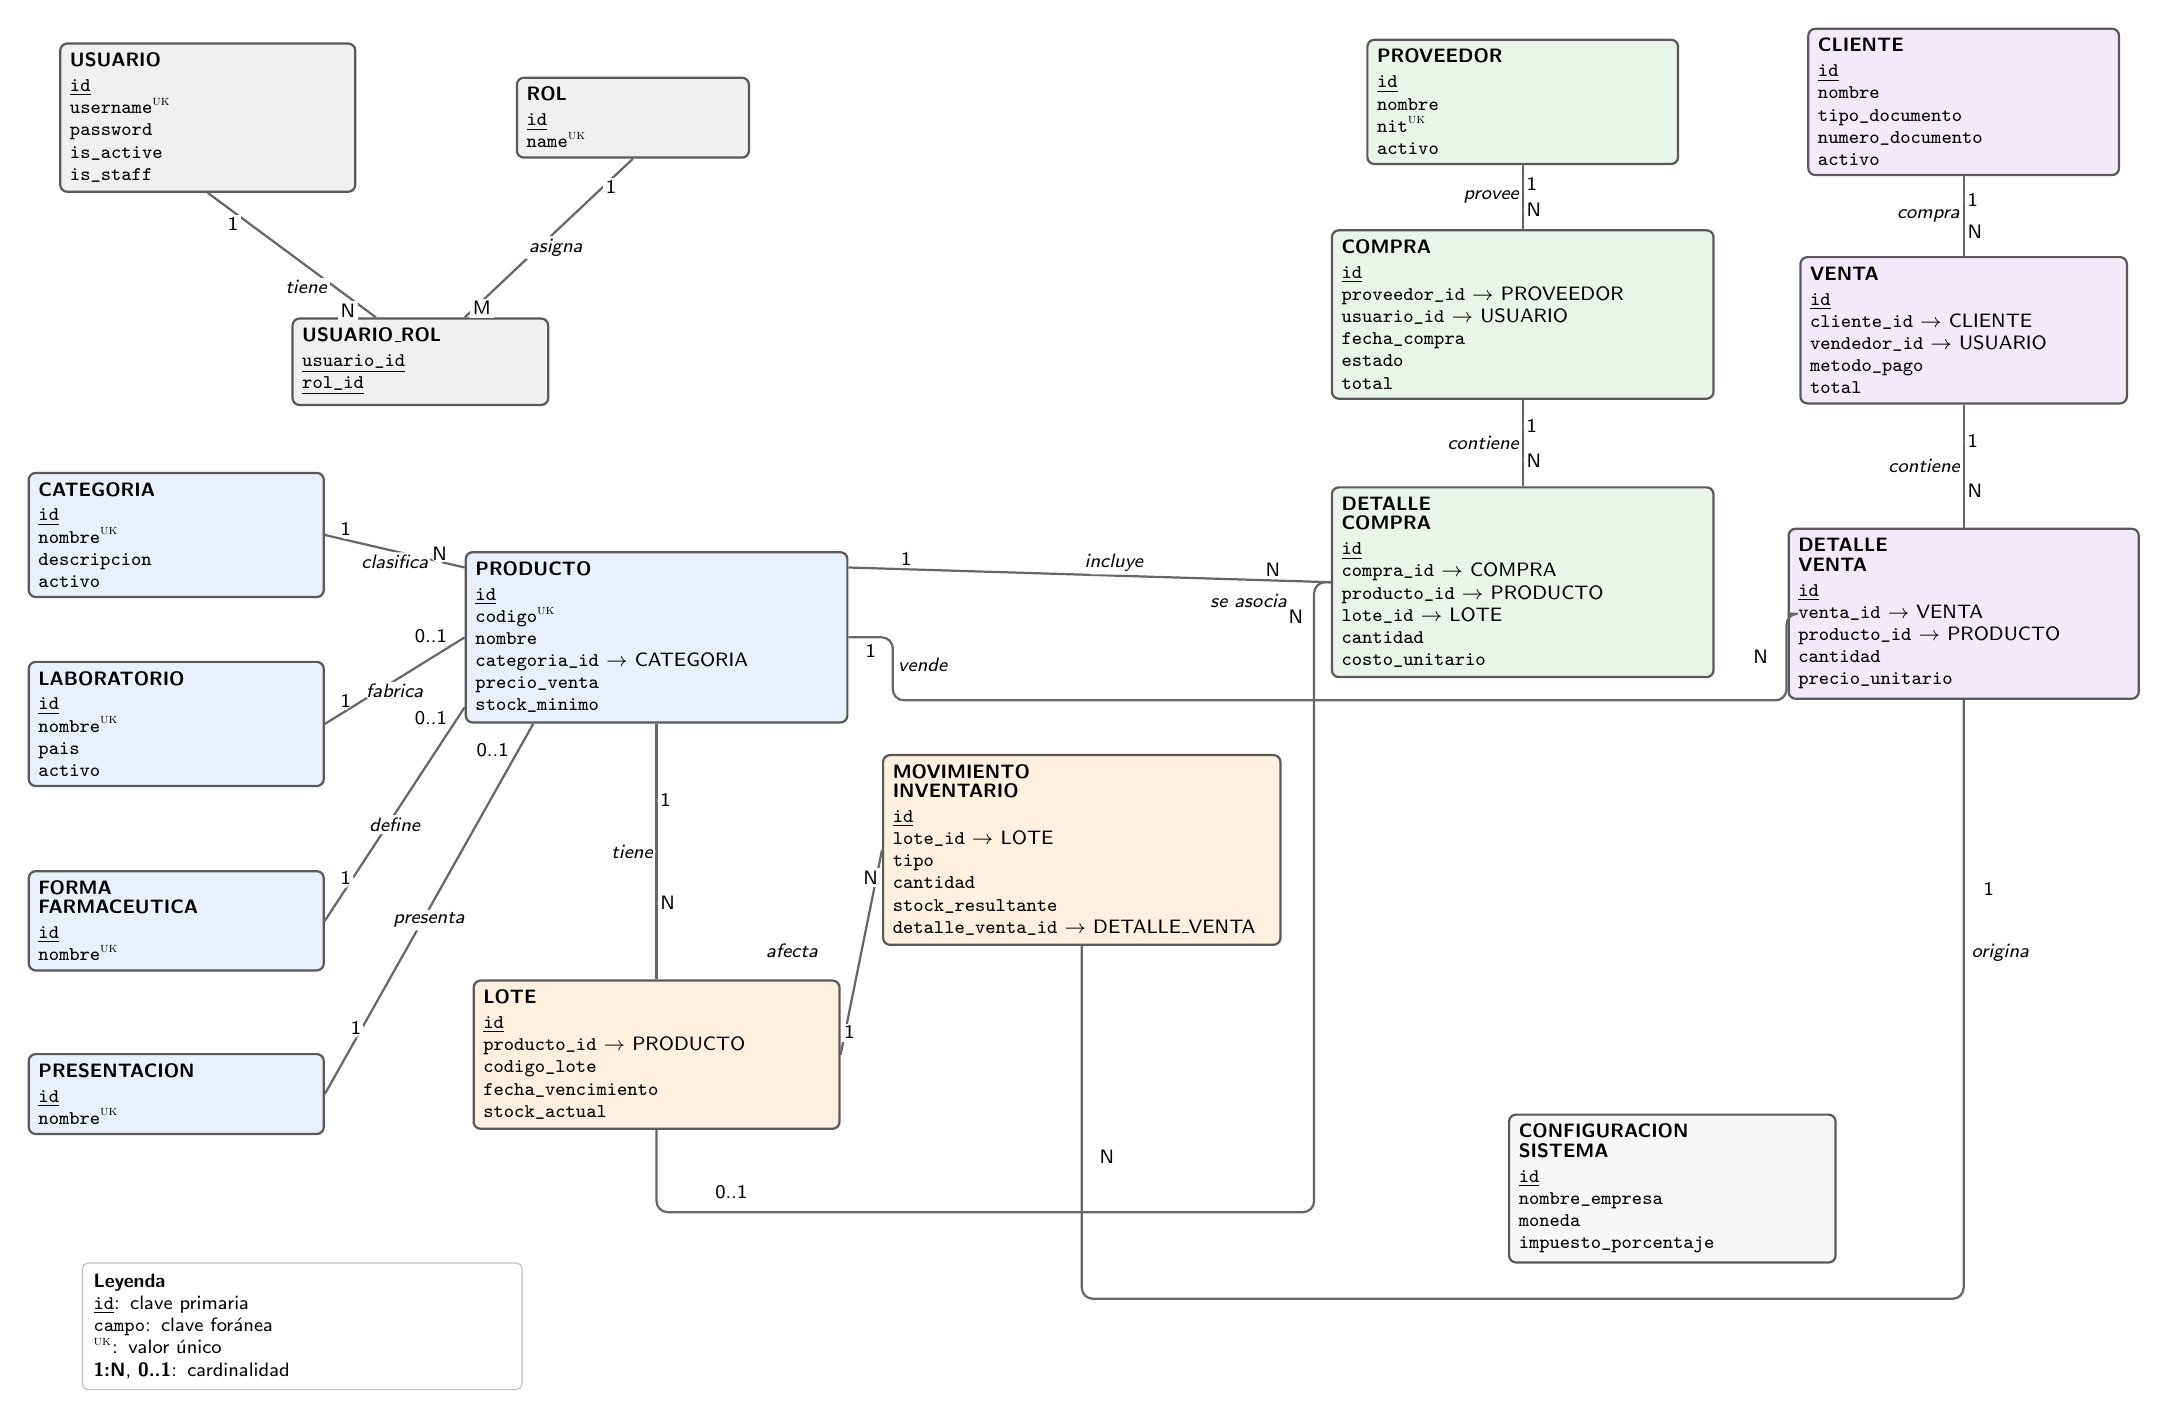
\begin{tikzpicture}[x=1cm,y=1cm]

% ------------------------- Seguridad -------------------------------------
\node[seguridad, text width=3.5cm] (usuario) at (3.3,16.2) {%
  \textbf{USUARIO}\\[1pt]
  \pk{id}\\
  \code{username}\uk\\
  \code{password}\\
  \code{is_active}\\
  \code{is_staff}
};

\node[seguridad, text width=2.7cm] (rol) at (8.7,16.2) {%
  \textbf{ROL}\\[1pt]
  \pk{id}\\
  \code{name}\uk
};

\node[seguridad, text width=3.0cm] (usuario_rol) at (6.0,13.1) {%
  \textbf{USUARIO\_ROL}\\[1pt]
  \pk{usuario_id}\\
  \pk{rol_id}
};

\draw[rel] (usuario.south) -- (usuario_rol.135);
\node[card] at (3.62,14.85) {1};
\node[card] at (5.08,13.75) {N};
\node[lbl] at (4.55,14.05) {tiene};

\draw[rel] (rol.south) -- (usuario_rol.45);
\node[card] at (8.42,15.32) {1};
\node[card] at (6.78,13.78) {M};
\node[lbl] at (7.72,14.55) {asigna};

% ------------------------- Catálogo --------------------------------------
\node[catalogo, text width=3.5cm] (categoria) at (2.9,10.9) {%
  \textbf{CATEGORIA}\\[1pt]
  \pk{id}\\
  \code{nombre}\uk\\
  \code{descripcion}\\
  \code{activo}
};

\node[catalogo, text width=3.5cm] (laboratorio) at (2.9,8.5) {%
  \textbf{LABORATORIO}\\[1pt]
  \pk{id}\\
  \code{nombre}\uk\\
  \code{pais}\\
  \code{activo}
};

\node[catalogo, text width=3.5cm] (forma) at (2.9,6.0) {%
  \textbf{FORMA}\\[-1pt]
  \textbf{FARMACEUTICA}\\[1pt]
  \pk{id}\\
  \code{nombre}\uk
};

\node[catalogo, text width=3.5cm] (presentacion) at (2.9,3.8) {%
  \textbf{PRESENTACION}\\[1pt]
  \pk{id}\\
  \code{nombre}\uk
};

\node[catalogo, text width=4.6cm] (producto) at (9.0,9.6) {%
  \textbf{PRODUCTO}\\[1pt]
  \pk{id}\\
  \code{codigo}\uk\\
  \code{nombre}\\
  \fk{categoria_id} $\rightarrow$ CATEGORIA\\
  \code{precio_venta}\\
  \code{stock_minimo}
};

\draw[rel] (categoria.east) -- (producto.160)
  node[pos=0.15, above, card] {1}
  node[pos=0.90, above left, card] {N}
  node[pos=0.50, below, lbl] {clasifica};

\draw[rel] (laboratorio.east) -- (producto.180)
  node[pos=0.15, above, card] {1}
  node[pos=0.90, above left, card] {0..1}
  node[pos=0.50, below, lbl] {fabrica};

\draw[rel] (forma.east) -- (producto.200)
  node[pos=0.15, above, card] {1}
  node[pos=0.90, above left, card] {0..1}
  node[pos=0.50, below, lbl] {define};

\draw[rel] (presentacion.east) -- (producto.215)
  node[pos=0.15, above, card] {1}
  node[pos=0.90, above left, card] {0..1}
  node[pos=0.50, below, lbl] {presenta};

% ------------------------- Inventario ------------------------------------
\node[inventario, text width=4.4cm] (lote) at (9.0,4.3) {%
  \textbf{LOTE}\\[1pt]
  \pk{id}\\
  \fk{producto_id} $\rightarrow$ PRODUCTO\\
  \code{codigo_lote}\\
  \code{fecha_vencimiento}\\
  \code{stock_actual}
};

\node[inventario, text width=4.8cm] (movimiento) at (14.4,6.9) {%
  \textbf{MOVIMIENTO}\\[-1pt]
  \textbf{INVENTARIO}\\[1pt]
  \pk{id}\\
  \fk{lote_id} $\rightarrow$ LOTE\\
  \code{tipo}\\
  \code{cantidad}\\
  \code{stock_resultante}\\
  \fk{detalle_venta_id} $\rightarrow$ DETALLE\_VENTA
};

\draw[rel] (producto.south) -- (lote.north)
  node[pos=0.30, right, card] {1}
  node[pos=0.70, right, card] {N}
  node[pos=0.50, left, lbl] {tiene};

\draw[rel] (lote.east) -- (movimiento.west);
\node[card] at (11.45,4.58) {1};
\node[card] at (11.72,6.55) {N};
\node[lbl] at (10.72,5.62) {afecta};

% ------------------------- Compras ---------------------------------------
\node[compras, text width=3.7cm] (proveedor) at (20.0,16.4) {%
  \textbf{PROVEEDOR}\\[1pt]
  \pk{id}\\
  \code{nombre}\\
  \code{nit}\uk\\
  \code{activo}
};

\node[compras, text width=4.6cm] (compra) at (20.0,13.7) {%
  \textbf{COMPRA}\\[1pt]
  \pk{id}\\
  \fk{proveedor_id} $\rightarrow$ PROVEEDOR\\
  \fk{usuario_id} $\rightarrow$ USUARIO\\
  \code{fecha_compra}\\
  \code{estado}\\
  \code{total}
};

\node[compras, text width=4.6cm] (detalle_compra) at (20.0,10.3) {%
  \textbf{DETALLE}\\[-1pt]
  \textbf{COMPRA}\\[1pt]
  \pk{id}\\
  \fk{compra_id} $\rightarrow$ COMPRA\\
  \fk{producto_id} $\rightarrow$ PRODUCTO\\
  \fk{lote_id} $\rightarrow$ LOTE\\
  \code{cantidad}\\
  \code{costo_unitario}
};

\draw[rel] (proveedor.south) -- (compra.north)
  node[pos=0.30, right, card] {1}
  node[pos=0.70, right, card] {N}
  node[pos=0.50, left, lbl] {provee};

\draw[rel] (compra.south) -- (detalle_compra.north)
  node[pos=0.30, right, card] {1}
  node[pos=0.70, right, card] {N}
  node[pos=0.50, left, lbl] {contiene};

\draw[rel] (producto.20) -- (detalle_compra.west)
  node[pos=0.12, above, card] {1}
  node[pos=0.88, above, card] {N}
  node[pos=0.55, above, lbl] {incluye};

% ------------------------- Ventas ----------------------------------------
\node[ventas, text width=3.7cm] (cliente) at (25.6,16.4) {%
  \textbf{CLIENTE}\\[1pt]
  \pk{id}\\
  \code{nombre}\\
  \code{tipo_documento}\\
  \code{numero_documento}\\
  \code{activo}
};

\node[ventas, text width=3.9cm] (venta) at (25.6,13.5) {%
  \textbf{VENTA}\\[1pt]
  \pk{id}\\
  \fk{cliente_id} $\rightarrow$ CLIENTE\\
  \fk{vendedor_id} $\rightarrow$ USUARIO\\
  \code{metodo_pago}\\
  \code{total}
};

\node[ventas, text width=4.2cm] (detalle_venta) at (25.6,9.9) {%
  \textbf{DETALLE}\\[-1pt]
  \textbf{VENTA}\\[1pt]
  \pk{id}\\
  \fk{venta_id} $\rightarrow$ VENTA\\
  \fk{producto_id} $\rightarrow$ PRODUCTO\\
  \code{cantidad}\\
  \code{precio_unitario}
};

\draw[rel] (cliente.south) -- (venta.north)
  node[pos=0.30, right, card] {1}
  node[pos=0.70, right, card] {N}
  node[pos=0.50, left, lbl] {compra};

\draw[rel] (venta.south) -- (detalle_venta.north)
  node[pos=0.30, right, card] {1}
  node[pos=0.70, right, card] {N}
  node[pos=0.50, left, lbl] {contiene};

% ------------------------- Configuración ---------------------------------
\node[configuracion, text width=3.9cm] (config) at (21.9,2.6) {%
  \textbf{CONFIGURACION}\\[-1pt]
  \textbf{SISTEMA}\\[1pt]
  \pk{id}\\
  \code{nombre_empresa}\\
  \code{moneda}\\
  \code{impuesto_porcentaje}
};

% ------------------- Relaciones con recorrido ortogonal ------------------
% PRODUCTO 1:N DETALLE_VENTA (canal entre detalle de compra y movimiento)
\draw[rel] (producto.east) -- (12.0,9.6)
  -- (12.0,8.8)
  -- (23.35,8.8)
  -- (23.35,9.9)
  -- (detalle_venta.west);
\node[card] at (11.72,9.42) {1};
\node[lbl] at (12.38,9.25) {vende};
\node[card] at (23.02,9.35) {N};

% DETALLE_COMPRA N:1 LOTE (recorrido inferior)
\draw[rel] (detalle_compra.west) -- (17.35,10.3)
  -- (17.35,2.3)
  -- (9.0,2.3)
  -- (lote.south);
\node[card] at (17.12,9.86) {N};
\node[lbl] at (16.52,10.06) {se asocia};
\node[card] at (9.95,2.56) {0..1};

% DETALLE_VENTA 1:N MOVIMIENTO (recorrido inferior)
\draw[rel] (detalle_venta.south) -- (25.6,1.2)
  -- (14.4,1.2)
  -- (movimiento.south);
\node[card] at (25.92,6.4) {1};
\node[lbl, right] at (25.66,5.6) {origina};
\node[card] at (14.72,3.0) {N};

% Leyenda dentro del área del diagrama
\node[draw=black!25, rounded corners=2pt, fill=white, font=\sffamily\scriptsize,
      align=left, inner sep=4pt, text width=5.3cm] at (4.5,0.85) {%
  \textbf{Leyenda}\\
  \pk{id}: clave primaria\\
  \fk{campo}: clave foránea\\
  \uk: valor único\\
  \textbf{1:N}, \textbf{0..1}: cardinalidad
};

\end{tikzpicture}%
}
\caption{Modelo entidad-relación de Farmacia Lufar. Las referencias de auditoría desde \code{USUARIO} hacia \code{CLIENTE}, \code{COMPRA}, \code{VENTA} y \code{MOVIMIENTO_INVENTARIO} se detallan en el modelo relacional para no saturar el diagrama.}
\label{fig:er}
\end{figure}

\subsection*{Cardinalidades principales}

\begin{center}
\small
\begin{tabular}{@{}ll@{}}
\toprule
\textbf{Relación} & \textbf{Cardinalidad} \\
\midrule
\code{CATEGORIA} -- \code{PRODUCTO} & 1:N \\
\code{PRODUCTO} -- \code{LOTE} & 1:N \\
\code{LOTE} -- \code{MOVIMIENTO_INVENTARIO} & 1:N \\
\code{PROVEEDOR} -- \code{COMPRA} & 1:N \\
\code{COMPRA} -- \code{DETALLE_COMPRA} & 1:N \\
\code{LOTE} -- \code{DETALLE_COMPRA} & 1:N (lote opcional en el detalle) \\
\code{CLIENTE} -- \code{VENTA} & 1:N (cliente opcional en la venta) \\
\code{VENTA} -- \code{DETALLE_VENTA} & 1:N \\
\code{PRODUCTO} -- \code{DETALLE_VENTA} & 1:N \\
\code{DETALLE_VENTA} -- \code{MOVIMIENTO_INVENTARIO} & 1:N \\
\code{USUARIO} -- \code{ROL} & N:M mediante \code{USUARIO_ROL} \\
\bottomrule
\end{tabular}
\end{center}

% ---------------------------------------------------------------------------
\section{Modelo relacional}

\subsection*{Convenciones}

En las relaciones se usa \pk{id} para la clave primaria, \fk{campo} para la clave foránea y \uk{} para los valores únicos. Las flechas $\rightarrow$ indican la relación referenciada. Los campos marcados como opcionales pueden ser \code{NULL}.

\begin{small}
\begin{longtable}{@{}>{\raggedright\arraybackslash}p{4.1cm}>{\raggedright\arraybackslash}p{22.0cm}@{}}
\toprule
\textbf{Relación} & \textbf{Atributos, claves y referencias} \\
\midrule
\endfirsthead

\toprule
\textbf{Relación} & \textbf{Atributos, claves y referencias} \\
\midrule
\endhead

\bottomrule
\endlastfoot

\multicolumn{2}{@{}l}{\textbf{\sffamily Módulo de seguridad (Django)}}\\
\addlinespace
\code{USUARIO} &
\pk{id}, \code{username}\uk, \code{password}, \code{first_name}, \code{last_name}, \code{email}, \code{is_active}, \code{is_staff}, \code{is_superuser}.\\
\addlinespace
\code{ROL} &
\pk{id}, \code{name}\uk.\\
\addlinespace
\code{USUARIO_ROL} &
\pk{usuario_id} $\rightarrow$ \code{USUARIO.id}, \pk{rol_id} $\rightarrow$ \code{ROL.id}. Clave primaria compuesta y unicidad de la pareja.\\
\addlinespace
\multicolumn{2}{@{}l}{\textbf{\sffamily Módulo de catálogo}}\\
\addlinespace
\code{CATEGORIA} &
\pk{id}, \code{nombre}\uk, \code{descripcion}, \code{activo}.\\
\addlinespace
\code{LABORATORIO} &
\pk{id}, \code{nombre}\uk, \code{pais}, \code{activo}.\\
\addlinespace
\code{FORMA_FARMACEUTICA} &
\pk{id}, \code{nombre}\uk.\\
\addlinespace
\code{PRESENTACION} &
\pk{id}, \code{nombre}\uk.\\
\addlinespace
\code{PRODUCTO} &
\pk{id}, \code{codigo}\uk, \code{nombre}, \code{descripcion}, \code{principio_activo}, \fk{categoria_id} $\rightarrow$ \code{CATEGORIA.id}, \fk{laboratorio_id} $\rightarrow$ \code{LABORATORIO.id} (opcional), \fk{forma_farmaceutica_id} $\rightarrow$ \code{FORMA_FARMACEUTICA.id} (opcional), \fk{presentacion_id} $\rightarrow$ \code{PRESENTACION.id} (opcional), \code{concentracion}, \code{unidad_medida}, \code{precio_venta}, \code{stock_minimo}, \code{activo}, \code{creado_en}, \code{actualizado_en}.\\
\addlinespace
\multicolumn{2}{@{}l}{\textbf{\sffamily Módulo de compras}}\\
\addlinespace
\code{PROVEEDOR} &
\pk{id}, \code{nombre}, \code{nit}\uk{} (opcional), \code{telefono}, \code{email}, \code{direccion}, \code{contacto}, \code{activo}, \code{creado_en}, \code{actualizado_en}.\\
\addlinespace
\code{COMPRA} &
\pk{id}, \fk{proveedor_id} $\rightarrow$ \code{PROVEEDOR.id}, \fk{usuario_id} $\rightarrow$ \code{USUARIO.id}, \code{numero_factura}, \code{fecha_compra}, \code{fecha_recepcion} (opcional), \code{estado}, \code{subtotal}, \code{impuesto}, \code{total}, \code{observaciones}, \code{creado_en}, \code{actualizado_en}.\\
\addlinespace
\code{DETALLE_COMPRA} &
\pk{id}, \fk{compra_id} $\rightarrow$ \code{COMPRA.id}, \fk{producto_id} $\rightarrow$ \code{PRODUCTO.id}, \fk{lote_id} $\rightarrow$ \code{LOTE.id} (opcional hasta la recepción), \code{cantidad}, \code{costo_unitario}, \code{subtotal}.\\
\addlinespace
\multicolumn{2}{@{}l}{\textbf{\sffamily Módulo de inventario}}\\
\addlinespace
\code{LOTE} &
\pk{id}, \fk{producto_id} $\rightarrow$ \code{PRODUCTO.id}, \code{codigo_lote}, \code{fecha_fabricacion} (opcional), \code{fecha_vencimiento} (opcional), \code{fecha_ingreso}, \code{stock_actual}, \code{activo}. Único por \code{(producto_id, codigo_lote)}.\\
\addlinespace
\code{MOVIMIENTO_INVENTARIO} &
\pk{id}, \fk{lote_id} $\rightarrow$ \code{LOTE.id}, \code{tipo}, \code{cantidad}, \code{stock_resultante}, \fk{detalle_venta_id} $\rightarrow$ \code{DETALLE_VENTA.id} (opcional), \code{motivo}, \fk{usuario_id} $\rightarrow$ \code{USUARIO.id}, \code{fecha}.\\
\addlinespace
\multicolumn{2}{@{}l}{\textbf{\sffamily Módulo de clientes y ventas}}\\
\addlinespace
\code{CLIENTE} &
\pk{id}, \code{nombre}, \code{tipo_documento}, \code{numero_documento}, \code{telefono}, \code{activo}, \fk{creado_por_id} $\rightarrow$ \code{USUARIO.id} (opcional), \code{creado_en}, \code{actualizado_en}. Único por \code{(tipo_documento, numero_documento)} cuando ambos no están vacíos.\\
\addlinespace
\code{VENTA} &
\pk{id}, \fk{cliente_id} $\rightarrow$ \code{CLIENTE.id} (opcional), \fk{vendedor_id} $\rightarrow$ \code{USUARIO.id}, \code{metodo_pago}, \code{monto_recibido}, \code{total}, \code{creado_en}.\\
\addlinespace
\code{DETALLE_VENTA} &
\pk{id}, \fk{venta_id} $\rightarrow$ \code{VENTA.id}, \fk{producto_id} $\rightarrow$ \code{PRODUCTO.id}, \code{codigo_producto}, \code{nombre_producto}, \code{cantidad}, \code{precio_unitario}, \code{creado_en}. Único por \code{(venta_id, producto_id)}.\\
\addlinespace
\multicolumn{2}{@{}l}{\textbf{\sffamily Módulo de configuración}}\\
\addlinespace
\code{CONFIGURACION_SISTEMA} &
\pk{id}, \code{nombre_empresa}, \code{nit}, \code{direccion}, \code{telefono}, \code{email}, \code{moneda}, \code{impuesto_porcentaje}, \code{logo}, \code{stock_minimo_default}, \code{actualizado_en}. Una sola fila lógica (\code{id = 1}).\\
\addlinespace
\end{longtable}
\end{small}

\subsection*{Restricciones de integridad}

\begin{enumerate}[leftmargin=*, itemsep=2pt]
  \item \code{LOTE.stock_actual >= 0} y \code{MOVIMIENTO_INVENTARIO.stock_resultante >= 0}. No se permite stock negativo.
  \item \code{PRODUCTO.precio_venta >= 0}, \code{PRODUCTO.stock_minimo >= 0}, \code{DETALLE_COMPRA.cantidad > 0}, \code{DETALLE_COMPRA.costo_unitario >= 0}.
  \item \code{VENTA.total >= 0} y \code{VENTA.monto_recibido >= VENTA.total}. La venta se registra solo en efectivo.
  \item \code{DETALLE_VENTA.cantidad} entre 1 y 9999; \code{DETALLE_VENTA.precio_unitario >= 0}.
  \item \code{DETALLE_VENTA} conserva \code{codigo_producto}, \code{nombre_producto} y \code{precio_unitario} como copia histórica.
  \item \code{COMPRA.estado} solo puede ser \code{BORRADOR}, \code{RECIBIDA} o \code{ANULADA}. Solo \code{RECIBIDA} genera movimientos de entrada.
  \item \code{MOVIMIENTO_INVENTARIO.tipo} solo puede ser \code{INICIAL}, \code{ENTRADA}, \code{SALIDA}, \code{AJUSTE_POSITIVO} o \code{AJUSTE_NEGATIVO}.
  \item \code{CLIENTE} exige que \code{tipo_documento} y \code{numero_documento} se registren juntos, o ambos vacíos.
  \item \code{LOTE} es único por \code{(producto_id, codigo_lote)}. Los lotes vencidos o inactivos no se usan para vender.
  \item Las operaciones que afectan varias tablas (venta + inventario, recepción de compra + inventario) se ejecutan dentro de \code{transaction.atomic()}.
\end{enumerate}

\subsection*{Índices recomendados}

\begin{center}
\small
\begin{tabular}{@{}ll@{}}
\toprule
\textbf{Tabla} & \textbf{Índice} \\
\midrule
\code{PRODUCTO} & \code{(codigo)} único, \code{(nombre)}, \code{(categoria_id)} \\
\code{LOTE} & \code{(producto_id, codigo_lote)} único, \code{(producto_id, fecha_vencimiento)} \\
\code{COMPRA} & \code{(fecha_compra)}, \code{(proveedor_id)}, \code{(estado)} \\
\code{VENTA} & \code{(creado_en)}, \code{(cliente_id)}, \code{(vendedor_id)} \\
\code{DETALLE_VENTA} & \code{(venta_id)}, \code{(producto_id)} \\
\code{MOVIMIENTO_INVENTARIO} & \code{(lote_id, fecha)}, \code{(fecha)} \\
\bottomrule
\end{tabular}
\end{center}

\subsection*{Correspondencia con las aplicaciones Django}

\begin{center}
\small
\begin{tabular}{@{}ll@{}}
\toprule
\textbf{App} & \textbf{Tablas propuestas} \\
\midrule
\code{accounts} & \code{USUARIO}, \code{ROL}, \code{USUARIO_ROL} (tablas de Django) \\
\code{catalogo} & \code{CATEGORIA}, \code{LABORATORIO}, \code{FORMA_FARMACEUTICA}, \code{PRESENTACION}, \code{PRODUCTO} \\
\code{compras} & \code{PROVEEDOR}, \code{COMPRA}, \code{DETALLE_COMPRA} \\
\code{inventario} & \code{LOTE}, \code{MOVIMIENTO_INVENTARIO} \\
\code{clientes} & \code{CLIENTE} \\
\code{ventas} & \code{VENTA}, \code{DETALLE_VENTA} \\
\code{core} & \code{CONFIGURACION_SISTEMA} \\
\code{reportes} & Sin tablas propias: consultas de solo lectura \\
\bottomrule
\end{tabular}
\end{center}

\subsection*{Orden de implementación}

\begin{enumerate}[leftmargin=*, itemsep=2pt]
  \item \textbf{Catálogo:} crear \code{CATEGORIA} y los catálogos opcionales; ampliar \code{PRODUCTO}. Para los productos existentes, crear una categoría ``General'' en una migración de datos.
  \item \textbf{Inventario:} crear \code{LOTE} y \code{MOVIMIENTO_INVENTARIO}. El movimiento puede referenciar \code{ventas.DETALLE_VENTA}; no crear la relación inversa desde ventas hacia inventario.
  \item \textbf{Compras:} crear \code{PROVEEDOR}, \code{COMPRA} y \code{DETALLE_COMPRA}; \code{DETALLE_COMPRA.lote_id} referencia \code{inventario.LOTE}.
  \item \textbf{Ventas:} integrar el servicio de inventario en \code{registrar_venta} para generar salidas FEFO. No se requieren cambios estructurales en \code{VENTA} ni en \code{DETALLE_VENTA}.
  \item \textbf{Configuración:} agregar \code{CONFIGURACION_SISTEMA} solo si se implementa el módulo de configuraciones.
  \item \textbf{Reportes:} implementar consultas sobre ventas, compras, lotes y movimientos; no crear tablas.
\end{enumerate}

\subsection*{Simplificación si no se confirman lotes}

Si la entrevista descarta el control por lotes y vencimientos, se puede usar una versión más simple:

\begin{itemize}[leftmargin=*, itemsep=2pt]
  \item Eliminar \code{LOTE}.
  \item Agregar \code{PRODUCTO.stock_actual} o una tabla \code{EXISTENCIA_PRODUCTO(producto_id, cantidad_actual, stock_minimo)}.
  \item Cambiar \code{MOVIMIENTO_INVENTARIO.lote_id} por \code{producto_id}.
  \item Quitar \code{DETALLE_COMPRA.lote_id}.
\end{itemize}

Se recomienda conservar \code{MOVIMIENTO_INVENTARIO}, porque permite auditar entradas, salidas y ajustes aunque no se usen lotes.

\end{document}
